\documentclass[conference]{IEEEtran}
\IEEEoverridecommandlockouts
% The preceding line is only needed to identify funding in the first footnote. If that is unneeded, please comment it out.
\usepackage{cite}
\usepackage{amsmath,amssymb,amsfonts}
\usepackage{algorithmic}
\usepackage{graphicx}
\usepackage{textcomp}
\usepackage{xcolor}
\usepackage{geometry}
\usepackage{float}
\usepackage{adjustbox}

\usepackage{biblatex} %Imports biblatex package
\addbibresource{references.bib}
\graphicspath{ {./Images/} }

\begin{document} 
\title{
A Study Into The Applications of Machine Learning in The Diagnosis \& The Prognostication of Breast Cancer\\
\vspace{5mm}
\large Department of Computing \\
\vspace{3mm} 
\large Letterkenny Institute of Technology \\
\vspace{3mm} 
\large Machine Learning
}
\vspace{3mm}  
\author{Ultan Kearns \& Liam Millar}
\maketitle
\begin{abstract}
    This paper aims to analyze which methods would be best suited to identifying factors which contribute to a cancer being malignant or benign and to predict the Diagnosis of breast cancer based on those factors. Machine Learning has been used in a variety of healthcare fields and has proven to be very successful in regards to automating / helping with certain tasks ranging from identifying similarities in different strains of DNA and making inferences on new DNA strains to diagnosing various types of diseases and predicting the prognosis from sample data.  Machine Learning is particularly useful when it comes to analyzing and comparing data, this data can then be used to train a model to notice certain similarities in malignant and benign tumours.  
    \\
    \\
    keywords - Machine Learning, Breast Cancer, Prognosis, Diagnosis
\end{abstract}

\section{Introduction}
Machine Learning is a field which aims to train machines to think and learn like humans. Machine Learning is a subset of AI which is comprised of many fields, and has been proven to perform very well in predicting outcomes in a large variety of areas such as STEM fields, Economics, Social Sciences and various others.  The ultimate goal of machine learning is to train a machine to perform a task without any human intervention and to learn to adapt to new data and new patterns which appear in the data.  There has been an increased reliance on machine learning in the past few years and it has become ubiquitous in the modern world.\\\\ For our purposes we trained models using our breast cancer data-set to start noticing patterns within the data. The models we trained were used to predict the diagnosis of Breast Cancer by analyzing features from our training data-set, we then used this model to predict the diagnosis values for our test set.  

As part of our research into how machine learning has been applied to cancer we discovered that an assortment techniques, including Artificial Neural Networks (ANNs) and Decision Trees (DTs) have been widely applied in cancer research for the development of quicker and more accurate screening methods and predictive models, with the aim of effective and accurate decision making as early as possible. Time is a major factor in obtaining a successful outcome in treatment. However although it is apparent that machine learning can be used to detect the indicators of cancer effectively, the impact of a misdiagnosis means a high degree of validation is required to review these methods if used in clinical environments.There are many ways which a machine may choose to learn we will explain the types of learning we used when trying this model in the upcoming sections.

\subsection{Supervised Learning}
During the course of this project we used supervised learning to train models to predict the diagnosis of breast cancer using labelled data.  After the models were trained using our training set we then tested them using the test set we had created. The test set included values from our data-set not present in our training sets. We used a variety of supervised learning methods to predict and analyze various aspects of our data, I will list the ones we used below. 
\vspace{2mm}
\subsubsection{Linear Regression}
This algorithm involves finding a line to best fit the data, this is achieved by modifying parameters to find the best fitting line for a given data-set. This method works by learning to predict a pattern within the data and drawing a line through a series of data points so that the line fits is close to as many of the points as possible, in this way we can make predictions by seeing how closely a given point would fit our line.  
\\
We used this method to determine how highly correlated certain features in our data-set were with the diagnosis.
\vspace{2mm}
\subsubsection{Naive Bayes}
Naive Bayes is a technique which makes features of an object have the same weight when trying to classify the data.  This algorithm works well on small data sets.  The model has some cons to it such as the zero frequency phenomenon which we will discuss in our Methodology section.  An example of Naive Bayes would be to train an image classifier for identifying cars, using Naive Bayes the property of a cars wheels would have just as much impact as the number of doors of the car.  The type of Naive Bayes we used in our notebook is called Gaussian Naive Bayes and assumes our data is in the shape of a Gaussian Curve, in other words normally distributed(think of a bell curve).

\subsubsection{Random Forest}
The random forest algorithm creates multiple decision trees based on different features in the data-set to determine whether a tumour is benign or malignant.  It first creates multiple trees then combines them into the final tree using the average of all predictions, we use the final tree to make our predictions.  We can also see the importance of each feature from it's GINI value.

\subsection{Unsupervised Learning}
We also used unsupervised learning techniques to analyze and classify our data.  Unsupervised learning works by analyzing commonalities in the data and clustering or grouping the data together.  Using unsupervised learning we hoped to train a model to divide or data-set into two groups Malignant \& Benign.

\subsubsection{K-Means}
K Means works be defining centroids within the data and determining how far away data points are from the centroids via a distance metric euclidean, Jaccardian, Manhattan etc.  The algorithm works by grouping the data in regards to how close they are to the centroids, the performance of this algorithm can be measured by the correctly predicted values and by a Silhouette Coefficient which is calculated by using the following equation \[(b - a) / max(a, b)\] where a is the intra-cluster distance(distance between data points in the cluster) and b is the inter-cluster distance(distance between clusters).  The Silhouette Coefficient gauges the performance of the model more accurately as it shows the results of our k value which could be too low or too high leading to inaccurate predictions.

\subsubsection{K Nearest Neighbour}
K Nearest Neighbour is an algorithm which measures the distance between data points by using a distance metric eg: Cosine distance, Euclidean distance, Jaccardian distance etc and groups data points which are near each other into clusters.  In K Nearest Neighbour we make the assumption that data points within a certain distance must have some common properties or features, in this way we can separate the data into groups which share these features.

\subsection{Breast Cancer}
Breast cancer is a type of cancer which forms in the breast tissue, it has many signs and symptoms such as: 
\begin{itemize}
    \item New lump in the breast or underarm (armpit).
    \item Thickening or swelling of part of the breast.
    \item Irritation or dimpling of breast skin.
    \item Redness or flaky skin in the nipple area or the breast.
    \item Pulling in of the nipple or pain in the nipple area.
    \item Nipple discharge other than breast milk, including blood.
    \item Any change in the size or the shape of the breast.
    \item Pain in any area of the breast.
\end{itemize} \cite{symptomsofbreastcancer}
\\
\\
Breast cancer is also one of the most common occurring cancers in women and the average risk of a woman developing cancer in her lifetime is about 13\% or 1/8 in the United States alone\cite{howcommonisbreastcancer} and in 2020 there were 2.3 million women diagnosed with the disease of which 685,000 succumbed to the disease\cite{breastcancerstatistics}. In Ireland 3,700 new cases of breast cancer are diagnosed each year\cite{breastcancerireland}. Breast cancer treatment is has a very high survival rate if caught early, the survival rate for those in high income countries was 90\% \cite{breastcancerstatistics}.
\subsection{Libraries we used in this project}
I have listed the libraries we have used in this project below:
\begin{itemize}
    \item numpy referred to throughout our notebook as np\cite{numpy}  - the Numpy library was used to perform numerical operations on our data-set
    \item pandas referred to throughout our notebook as pd \cite{pandas} - Pandas was used to create dataframes from our data-set
    \item sklearn referred to throughout our notebook as sk \cite{sklearn} - We used SKlearn to implement many of our models and to output statistics relating to the models.
    \item matplotlib \cite{matplotlib} - We Used the matplotlib library to create visual interpretations of our data
    \item google.colab \cite{googlecolab} - Google Colab was used to upload our data set and also as an editor so we could compile and run our Jupyter Notebook\cite{jupyter}
    \item pyresearch - used to compute the Cramérs V score of our regression models.
\end{itemize}
\subsection{Aims of the project}
 The aim of this project is to train a model using machine learning to analyze data from both benign and malignant tumours to detect patterns in the data and to predict whether tumours will be malignant or benign given certain parameters with reasonable accuracy.
\section{Methodology}
\subsection{Creating testing and training sets}
We created testing and training sets from the data set by splitting the data set using the Sklearn Library\cite{sklearn} and creating four data-frames two for our X \& Y test sets and two more for our X \& Y training sets.  We then used the training sets to train a variety of models to make predictions about our test sets, we then measured the models performance based on how accurately it predicted data in the test set.  We used a variety of metrics to compare our data when using different models and gauged how accurately they performed on our test data.  When deciding how we should split the data we experimented with a number of values to decide on which split best suited our models, we determined this through trial and error rerunning our models with different splits to determine which split yielded the most accurate prediction.  
\subsection{Cleaning The Data}
The data-set we used was the Breast Cancer Wisconsin (Diagnostic) \cite{misc_breast_cancer_wisconsin_17}. This data-set consists of features computed from digitized images of Fine Needle Aspirate (FNA) of breast mass. It contains 569 instances(rows) and 32 variables(cols). There are 2 categorical variables ID and Diagnosis(our target). There is also 30 continuous variables used to describe the features broken into 3 sets of ten measurements using different methods. There was no missing data in this set so no imputation methods needed to be used.
I have included an image below to show a positive correlation between the Mean Radius and Mean Perimeter columns.  We also changed the diagnosis columns from 'M' for malignant and 'B' for benign to 1 for malignant and 0 for benign, this made the data much easier to work with and helped us in performing various algorithms with it.
\begin{figure}[H] 
\caption{Example of a positive linear correlation between the mean radius \& perimeter, if the lines slope was the inverse of our current line that would be an example of high negative correlation and we would not have needed to remove these columns from our data set}
\centering
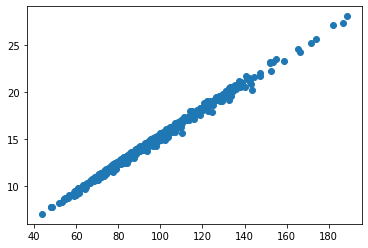
\includegraphics[height=50mm,width=0.5\textwidth]{positive_correlation.png}
\end{figure}
We were able to find this highly correlated data by using Pearson's correlation and I will include an image of the correlation in our data-set below
\begin{figure}[H]
\caption{Example of highly correlated variables in our data set as you can see the mean area corresponds highly with the data highlighted}
\centering
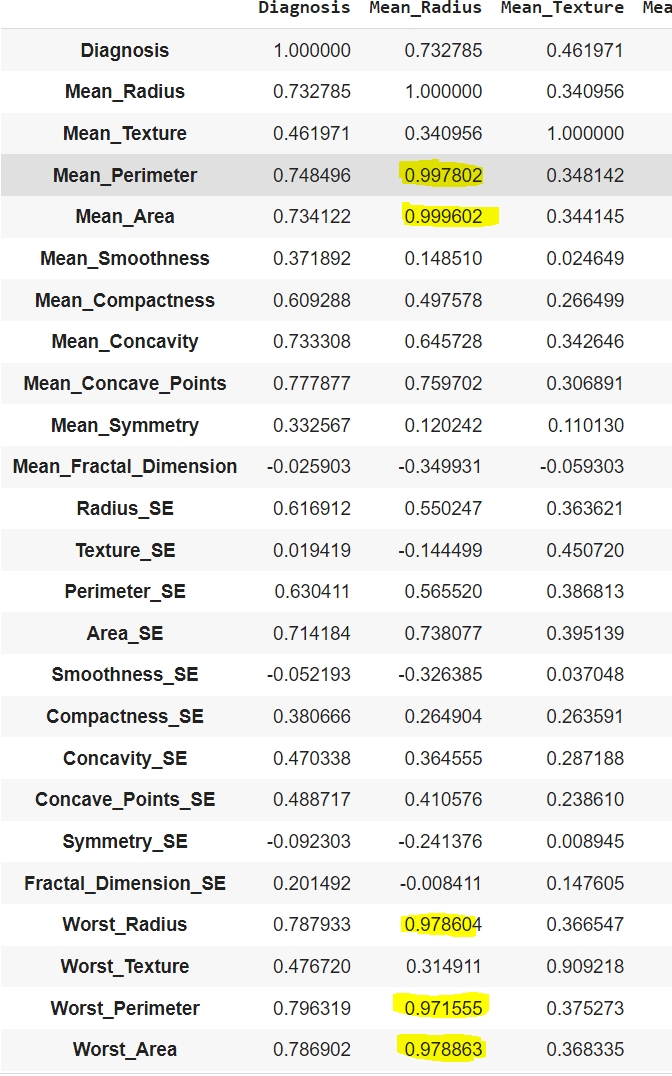
\includegraphics[height=80mm,width=0.5\textwidth]{dataset_correlation.PNG}
\end{figure}
Additionally we produced a heat-map of the correlations.
\begin{figure}[H]
\caption{The heat-map of correlations. This indicates a clear correlation between some of the columns and the complexity emphasises the need to reduce these columns where possible.}
\centering
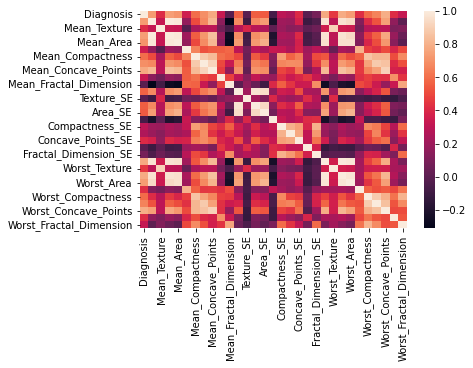
\includegraphics[height=60mm,width=0.5\textwidth]{correlation_heatmap.PNG}
\end{figure}
\subsection{Algorithms}
\subsubsection{Linear Regression}
In the notebook we used linear regression to predict values from our X test set based on features in the X training set.  We decided to use Diagnosis and Mean Area SE to verify the strength of the correlation.  Our dependent variable was the Diagnosis and our independent variable was the Mean Area SE.   We trained the model by first creating our X training set which contained the Mean Radius feature and then we created or X test set using the Mean Area we then reshaped the training and test data into a 2d array containing our feature values.  We then fit a model to display our results as we can see in the image below the relation between Mean Area SE and Diagnosis is positively correlated.  We also showed the Cramér's V value and P Value to see how correlated our variables were with each other to determine the impact the independent variable had on the dependent variable, our p-value for this model was 0.35 and our Cramérs V value was 0.98 indicating a fair amount of correlation and a high amount of association between our variables.  To compute the line we used this formula 
\begin{multline}
    Y_i = f(X_i,\beta) + e_i
\end{multline}
Where $Y_i$ is the dependent variable, $f$ symbolizes this is a function, $X_i$ is the dependent variable and $e_i$ is the error terms.
\
\begin{figure}[H]
\caption{Linear Regression Model of Mean Area\_SE and Diagnosis.}
\centering
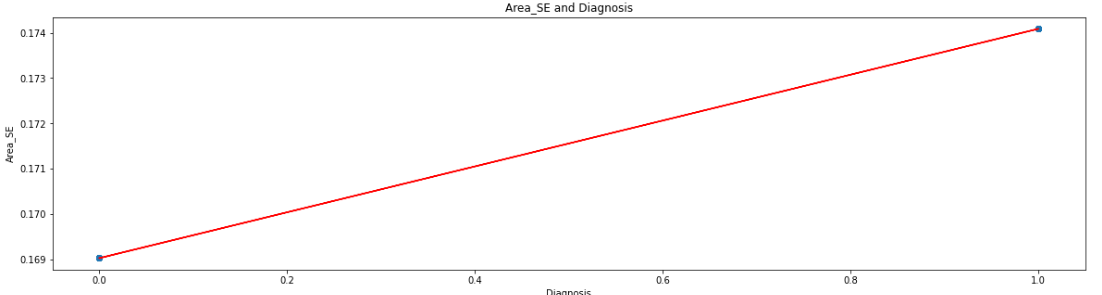
\includegraphics[height=60mm,width=0.5\textwidth]{Images/area_diagnosis.png}
\end{figure}
For our second linear regression model we decided to use Texture\_SE \& Diagnosis our independent variable was the Texture\_SE  which we used to predict the dependent variable which was the Diagnosis.  As you can see from the image below the data was more highly correlated and thus the values are higher than those in our first model.  Our p-value for this second model was 0.54 and our Cramérs V value was 0.96 indicating high correlation and high association between our variables.  The below image shows these variables have a negative correlation.
\begin{figure}[H]
\caption{Linear Regression Model of Texture Severity and Diagnosis.}
\centering
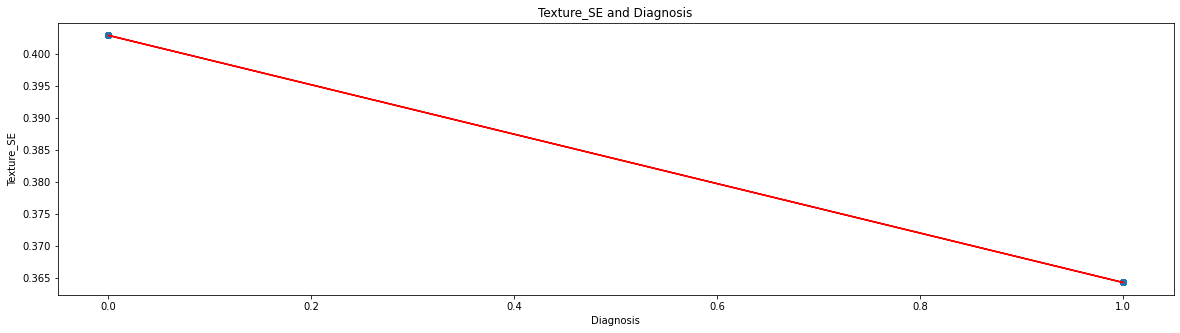
\includegraphics[height=60mm,width=0.5\textwidth]{Images/Texture_Diagnosis.png}
\end{figure}
\subsubsection{Decision Trees}
Decision Trees are a form of supervised learning that construct a flow chart from a set of training data and its results. This flow chart allows the prediction of future results based on a comparison to the features. However they can be prone to over fitting as all future decisions are based on the importance attributed to features of the training data. As part of our exploration of the data set we did a side by side comparison of decision trees based on information gain(entropy) and the Gini index(Gini) methods.
From our results we discovered that while both methods provided quite accurate results 0.90 or about 90.0\% for information gain and 0.93, or about 93.0\% for the Gini method. the scikit default Gini proved to be the most accurate.
\subsubsection{Random Forest} Random Forest is used to construct multiple decision trees from samples of the training data in order not to limit its scope and try to alleviate some of the issues with over fitting and precision that can occur with a single decision tree, this collection of trees produce separate predictions that are used as votes to form a majority decision on the final predicted result. We used the same data split to test using the random forests for both Gini and entropy(information gain), once again accuracy was high with 0.95 or 95\% for Gini and 0.94 0r 94\% for entropy, these values varied a little for the random forest due to the randomness but they remain consistently higher than the respective decision tree model and even the entropy random tree models accuracy improved upon the Gini singular decision tree. 
\subsubsection{Cross Validation} Because our data-set was reasonably small we ran some cross validation testing on the tree and random forest models 
\subsubsection{Naive Bayes}
We implemented Naive Bayes in our notebook by using all features from our training set as well as the diagnosis values in the y training set to train a model to predict the diagnosis of breast cancer.  We chose to use all features because in general the more features Naive Bayes has the more accurate the prediction.  When first implementing this algorithm we encountered an issue where the model would predict the same values over and over again.  We rectified this by scaling the data which ensured the model had a relatively even probability of predicting both malignant and benign.  The Naive Bayes model achieved a final score of 167 out of 171 or 97\% accuracy.
\subsubsection{K Nearest Neighbour}
We implemented K Nearest Neighbour by using our X train set which contained our training values and our y train set which contained our diagnosis values, the model was then fitted using the X and y training sets.  We chose a value of 55 for the neighbours we've passed in to the model as this yielded the best results.  We then tested the model by comparing values in our test array to the predicted values of our model, the model was right on average around 520 out of 569 times, giving it a ~95\% accuracy rating. The models accuracy changes with the test / training set split the values mentioned above were achieved using a 70/30 split.
\section{Challenges}
\subsection{Over fitting}
Over fitting occurs when the model is performing very well on the training data but performs poorly on new data, this is due to the fact that the model has been trained to fit the training data so well that it cannot adapt to different data. To try and alleviate this we performed dimensionality reduction to find the features that are discriminative.
\subsubsection{Principal Component Analysis(PCA)} This is a form of unsupervised dimensionality-reduction and as our data-set contained a high number of features 30 we also explored the possibility of reducing these features by finding principle components that retain the essential parts of the data with the most variation while eliminating the sections that had little variation and less essential. A number of the features we saw were highly correlative as they were  derived from each other such as radius, diameter and area of a circle. This implied that PCA was a good method of dimensionality reduction to explore. We standardised the data-set to remove the impact of diverse measurement scales. We experimented with a number of different dimensions but found that seven dimensions was a good compromise as it retained over 90\% of the data but reduced the features to less than a quarter. If speed was a factor with larger data we could consider a further reduction but we felt high data retention was important in a medical matter. The gini decision tree accuracy was 0.94 or 94\% and the Gini random forest was 0.97 or 97 \% with this arrangement.
\subsection{Under fitting}
When training the models we also had to worry about under-fitting the data, under-fitting occurs when the model does not predict well enough on either the training or test sets.  Such a model is not practical and has no purpose or uses.
\subsection{Naive Bayes}
The Naive Bayes model suffered from an issue in the beginning where it only predicted one value for all values in our data-set.  This may have been caused by a phenomenon known as zero frequency, which is where our data may not have had any malignant or benign labels, we rectified this by scaling the data and achieved fairly accurate of 158 / 171 or around 92\%
\section{Applications}
\subsection{Diagnosis of Breast Cancer}
The KNN model has a fairly accurate prediction of the diagnosis as does our first Naive Bayes model, as with all diagnostics tools there will need to be a doctor on hand also to analyze the information in case the AI generates false negatives or false positives.  The models do provide however an insight into whether a tumour is benign or malignant.
\subsection{Prognosis of Breast Cancer}
The models can predict whether a tumour will be malignant or benign from features in our data-set this means that doctors can feed in the values of said features and produce a prognosis indicating the possibility of the tumour being benign or malignant.  The models we included in this notebook can offer predictions on tumours being benign or malignant but these predictions should always be verified by a trained professional as some models can lead to false positives or much worse in our case, false negatives.  Machine Learning is very useful in the medical field but even the best trained models can yield false predictions.
\section{Conclusion}
\subsection{Accuracy of Models}
\begin{adjustbox}{max width=\textwidth}
\begin{tabular}{lr}

\hline
 Method Description                     &Accuracy\\
\hline
 PCA Gini Random Forest:                &0.98\%\\
 cross validation Gini rdm forest:   &0.96\%\\
 Standard trained Gini rdm forest:   &0.95\%\\
 cross validation Ent random forest:&0.95\%\\
 PCA Gini Tree:                         &0.94\%\\
 Standard trained Ent random forest:&0.94\%\\
 Standard trained Gini decision tree:   &0.94\%\\
 cross validation Ent decision tree:&0.92\%\\
 Gaussian Naive Bayes-with scaling:   &0.93\%\\
 Gaussian Naive Bayes-without scaling:&0.92\%\\
 Standard trained Ent decision tree:&0.91\%\\
 cross validation Gini decision tree:   &0.91\%\\
 K Neighbour:                           &0.90\%\\
 K Means:                               &0.86\%\\
 Gaussian Naive Bayes-with smoothing: &0.79\%\\

\hline
\end{tabular}
\end{adjustbox}
\\
\\
\subsubsection{Random Forest}
As we can see from the table above our most accurate model appears to be the Gini Random Forest using the Principal Components garnered during our analysis. Consistently the Random forest methods ranked highest using the different data arrangements we used.
\subsubsection{Gaussian Naive Bayes}
We included three Gaussian Naive Bayes models in our notebook, the first, second and third seem to predict fairly well although adjusting our train / test split can have an effect.  In our third Naive Bayes model we scaled the data is producing slightly better predictions due to the data being scaled.  Our first models suffered previously when performing predictions as we encountered the zero frequency problem, we adjusted the models and the issue was rectified.  Our  second Naive Bayes Model includes smoothing which had a negative effect on performance.
\subsubsection{KNN}
The KNN model predicts fairly accurately when the training / test split is 70/30, below I will include the correctly predicted values out of the actual values.

Total values:  171  correctly predicted values:  155 which is approximately 0.90\%

From the above results we can see that this technique works very well with our data set with around 9 / 10 predictions being accurate. 
\subsection{What could be done differently}
Our data-set was quite small which would lead to some concerns about over fitting for the training data especially for the likes of decision tree. We took steps to alleviate some of the concerns about this. For the purpose of our exercise this was fine but ideally an expanded set of real world data points for training would ensure a more confident outcome.
\subsection{In conclusion}
In conclusion we found that using the PCA Gini Random Forest model to be the best performing model in our notebook.  We also see that most of our models performed fairly with the lowest scoring 0.79\%.  We have found from our study that even the best performing models have margins of error, it is for this reason the that a doctor should always review the results of ML models.  By using these models as an assistant we hope to help doctors by alerting them to positive cases of breast cancer so that it can be caught early and the treatment prescribed will be more successful.
\newpage
\clearpage
\tableofcontents
\printbibliography
\listoffigures
\end{document}
